\def\theTopic{ Comparing Distributions }
\def\dayNum{10 }

\begin{center}
{\bf {\large Comparing Distributions}}
\end{center}

\begin{enumerate}
   \item  Suppose you are choosing which professor's class to enroll
     in.  You have three choices, and have data on the grade
     distribution for each. (Here grade is a percentage from 0 to 100,
     which is a {\bf quantitative} variable.  If we used letter
     grades, it would be a {\bf categorical} variable, telling us
     a letter--grade category for each student). Which class seems to
     have the best grade distribution? Explain why you prefer this one. 

    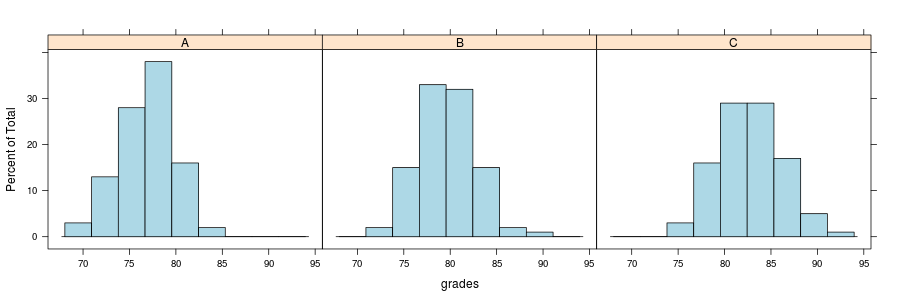
\includegraphics[width=.9\linewidth]{plots/3classGradeCompareMn.png}
\begin{students}
    \vspace{3cm}    
\end{students}

\begin{key}
  {\it Class C has the largest mean and largest median, so most will vote for it. }
\end{key}

\item  Here's another set of three distributions of exams scores.
     The density plots shown are essentially smoothed off histograms.
     Which do you prefer?  Explain why you prefer it. 

   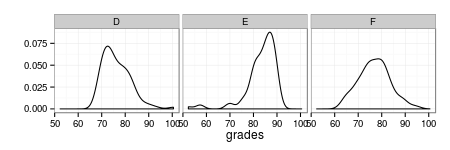
\includegraphics[width=.9\linewidth]{plots/3classGradeCompareSkw.png}
\begin{students}
    \vspace{5cm}    
\end{students}

\begin{key}
  {\it Class H has more A's than C's, so it's the wise choice.  I
    seems evenly split to high and low grades, while G seems to have
    lots of low grades.}
\end{key}
     
   \item  And here's a third set.  Which do you prefer?  Explain the
     differences.  
     
    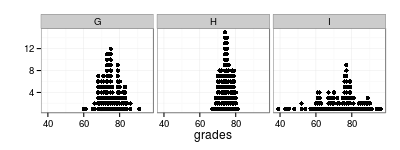
\includegraphics[width=.9\linewidth]{plots/3classGradeCompareSD.png}
\begin{students}
    \vspace{3cm}    
\end{students}

\begin{key}
  {\it The big difference here is in spread.  If you're an ``average''
  student, then you would like E because almost everyone gets a C and
  there's little chance of flunking.  If you are a good student, then
  F is more attractive since more people get A's in this class.}
\end{key}
  
  \item  When comparing distributions there are several things to consider:
    \begin{enumerate}
    \item  Comparing location or center (measured by mean or median)
      tells us which class did best ``on average''. 
    \item  Comparing spread (interquartile range or standard
      deviation) tells us which class is generally closest to its mean.
    \item  Comparing skew (could be left or right) to symmetric.
      Let's hope that there are more high grades than low ones. 
    \end{enumerate}
    In the three problems above, which comparison were you making?
    For each set of comparisons, fill in center, spread, or skew. \\
    1 
\begin{students}
\underline{\hspace*{3cm}}\hfill 
\end{students}
\begin{key}
  \underline{\hspace*{1cm}}  {\it  center} \underline{\hspace*{1cm}}\hfill 
\end{key} 
    2 
\begin{students}
   \underline{\hspace*{3cm}}\hfill 
\end{students}
\begin{key}
  \underline{\hspace*{1cm}}  {\it  skew} \underline{\hspace*{1cm}}\hfill 
\end{key}
    3 
\begin{students}
  \underline{\hspace*{3cm}}\hfill 
\end{students}
\begin{key}
  \underline{\hspace*{1cm}}  {\it spread} \underline{\hspace*{1cm}}\hfill 
\end{key}
  \item   Of the three comparisons above, which was easiest and which
    was hardest? Explain. 
\begin{students}
    \vspace{2cm}    
\end{students}

\begin{key}
  {\it  Center is generally the easiest.  One could argue that spread
    is hard because you have to read the scales carefully, plus it
    depends on your amount of ambition for a good grade.  Skew is also
  hard because it require a close comparison of each tail. In this
  case, lots of A's are clearly preferred to an even spread or to more
D's.}
\end{key}


  \item  Here's your chance to weigh in on the topic of patience.  Are
    men or women more patient with slow restaurant service?  Write
    down a consensus group opinion to focus us on our next
    task.
\begin{students}
    \vspace{2cm}    
\end{students}

\begin{key}
  {\it AWV}
\end{key}

  \item  Go to the web site given on D2L and answer the questions there.
  %%    {\footnotesize  \url{https://docs.google.com/forms/d/1hWjQcYgS3Hf4A54-tf9ypSFTX1FhUgnr2UsbdtXGKls/viewform}}   
 
    For the fast food questions, imagine that you are hungry and want
    something to eat right away.  In the second situation, you are out
    for dinner at a very nice restaurant with close friends whom
    you've not seen for several months. Each group member should enter
    his/her own values.  (Nothing to write here.)


  \begin{center}
    {\bf  Comparing Blood Pressures}
  \end{center}
\item  While we're waiting for everyone to enter their data, get
  acquainted with the Statkey tool \fbox{Descriptive Statistics for one
  Quantitative and one Categorical Variable}. Go to the site:\\
  \url{www.lock5stat.com/statkey} and we'll
  start by looking at their data.  
  
  Click the box for data name \fbox{Student Survey (TV watching by gender)}
  right under \fbox{Statkey} and switch to 
  \fbox{ICU Admissions (Blood pressure by status)}. 
  Examine the dotplots. The two groups are separated by
  whether the patient left ICU alive or left ICU by dying. We wonder
  if blood pressure at the patients’ entry to ICU tells us something
  about their outcome.  

  \begin{enumerate}
    \item How many people had blood pressure under 100?
\begin{students}
    \vspace{1cm}    
\end{students}

\begin{key}
  {\it 20. Seven more were right at 100.}
\end{key}


    \item What proportion of those in the low blood pressure group
      died in ICU? 
\begin{students}
    \vspace{1cm}    
\end{students}

\begin{key}
  {\it 13/20 = 65\%}
\end{key}

    \item How many people had blood pressure over 100?
\begin{students}
    \vspace{1cm}    
\end{students}

\begin{key}
  {\it  180}
\end{key}

    \item What proportion of those in the higher blood pressure group
      died in ICU?
\begin{students}
    \vspace{1cm}    
\end{students}

\begin{key}
  {\it 27/180 = 15\%}
\end{key}


  \end{enumerate}
\item  Click histogram and boxplot to get different views.  Describe
  and compare the distributions for the two groups of people (left
  alive or left by dying).  
  \begin{enumerate}
  \item Are the centers similar for the two groups? 
\begin{students}
    \vspace{1.5cm}    
\end{students}

\begin{key}
  {\it No. mean Bp of those who dies was 119, of those who lived, 136.
   Medians are even closer, 126 to 132.}
\end{key}


  \item Are the spreads similar? 
\begin{students}
    \vspace{2cm}    
\end{students}

\begin{key}
  {\it No, SD estimate is 30 for lived, 41 for those who died. IQR is
    44 for the lived group, 52 for those who died. }
\end{key}

  \item Are the distributions symmetric or skewed?
\begin{students}
    \vspace{2cm}    
\end{students}

\begin{key}
  {\it I'd say symmetric, but long tailed.}
\end{key}
  \end{enumerate}


  \begin{center}
    {\bf Comparing Wait Times}
  \end{center}
\item  Click \fbox{Edit Data} and delete all data in their example.  \\
    Go to the Google Doc spreadsheet (see link on D2L)  to see class
    responses from the  web data form.%%\\ {\footnotesize
%%    \url{https://docs.google.com/spreadsheet/ccc?key=0AsNevGGB3qradERkQWZQZGxvSkF2MnZ6SEkyUXE2LUE#gid=0}}

    At the bottom, click \fbox{Sheet 2} to get the data we need.
    Shift-drag over columns A and B and push CONTROL-C for copy. 

    Paste the data into the edit data box on StatKey.  If you get a
    data entry error, you may have to add a comma in each row after
    Male or Female.  Look at the dotplot, histogram, and
    boxplot.
    \begin{enumerate}
    \item  Sketch the boxplots here.
\begin{students}
    \vspace{2cm}    
\end{students}

\begin{key}
  \includegraphics[width=.6\linewidth]{plots/Wait4FoodBoxplots1.png}
\end{key}

    \item   Write down the means and medians for men and women.  Is
      there much difference between men and women?  
\begin{students}
    \vspace{2cm}    
\end{students}

\begin{key}
  {\it Medians: Males: 12.7, Females:14.6,\\
       Means:   Males:  15.00	Females: 13.00  seem pretty close, but
     note that order is opposite for means and medians.}
\end{key}


    \item Write down the standard deviations and IQR = Q3 -- Q1 for men
      and women.  Is it obvious that spread differs by gender?
\begin{students}
    \vspace{2cm}    
\end{students}

\begin{key}
  {\it  IQR: Men: 15-10 = 5, Women: 20 - 10 = 10.  I think the
    difference in spread is quite obvious.  }
\end{key}



    \item Describe the shape of the distributions. Does it vary by
      gender? Are there outliers in either group?  
\begin{students}
    \vspace{2cm}    
\end{students}

\begin{key}
  {\it  Each group has some outliers, but there are far more women who
  are not in a hurry than men. The longest time for women to wait is
  60 min, but it's 30 for men.}
\end{key}

    \end{enumerate}
    

  \item  A restaurant manager tries to keep customers happy so they
    don't write a scathing online review.  What's the longest wait
    time that would keep at least 50\% of customers happy? 90\%?
    95\%? 
\begin{students}
    \vspace{2cm}    
\end{students}

\begin{key}
  {\it The overall median is 15 minutes, so that would keep half the
  customers happy. The most impatient 10\% are at or below 5 minutes
  and 5 \% is 12 who want their food in 4 minutes. }
\end{key}


  \item  Column C of the spreadsheet contains yes or no for having
    experience in a fast food establishment and column D of the
    spreadsheet contains the amount of time between expected wait and
    getting bothered.  Copy these data into StatKey and compare the
    two distributions.  Is there much difference?
\begin{students}
    \vspace{5cm}    
\end{students}

\begin{key}
  {\it Mean, median and spread all match. A large majority have not
    worked in fast food.}

  \includegraphics[width=.6\linewidth]{plots/Wait4Food-2.png}

\end{key}


Comment on what you've found.  Do you think work experience makes any
difference in patience for wait time in getting fast food? How so? 
\begin{students}
    \vspace{\fill}    
\end{students}

\begin{key}
  {\it There is no discernable
    difference by experience. Everyone gets hungry and wants food in a
  hurry. }
\end{key}


\end{enumerate}






\begin{center}
  {\bf Take Home Message:}
\end{center}

We make comparisons every day.  When comparing distributions of data,
we often care about mean or median, but we may also care about the
spread of the distribution.  When data are highly skewed, a few
outliers make a big difference.  In the rest of this course we will be
comparing centers of distributions.  This is not appropriate unless
the distributions are of similar shape and spread, however, it is the
most commonly used comparison.  If you understand the principles used
to make statistical comparisons, you'll be able to easily modify them
for other types of comparisons such as comparing slopes when fitting
regression lines (take Stat 217 to learn more).  



